\section{The Sparse Matrix Class}\label{sec:sparsematrix}
A sparse matrix is an option to store matrices without compromising computational memory usage. Since the number of non-zero elements in a matrix is relatively lower than the total number of elements, the sparse matrix is a good choice. In this section, the SparseMatrix class is explained and, for the matrix A shown in Section \ref{sec:fullmatrix_implementation}, the memory usage is compared to the full matrix storage method.
\subsection{Class Implementation} \label{sec:sparsematrix_implementation}
SparseMatrix class' attributes are as follows by Code \ref{code:sparsematrix_attributes}:
\begin{lstlisting}[language=python, caption={SparseMatrix Class Attributes}, label={code:sparsematrix_attributes}]
@dataclass
class SparseMatrix:
    data: list = field(init=False, default_factory=list) # List of non-zero elements
    cols: list = field(init=False, default_factory=list) # List of columns
    ptr: list = field(init=False, default_factory=list) # List of cumulative sums of non-zero elements
    sparsity: float = field(init=False, default=0.0) # Sparsity of the matrix
    density: float = field(init=False, default=0.0) # Density of the matrix
    size: int = field(init=False, default=0) # Size of the full matrix

    data_memory: int = field(init=False, default=0) # Memory usage of the data list
    cols_memory: int = field(init=False, default=0)
    ptr_memory: int = field(init=False, default=0)
    total_memory: int = field(init=False, default=0)
\end{lstlisting}    
Among them, highlights the data, in which the non-zero elements are stored, cols, in which the column indexes of each non-zero element are stored, and ptr, in which the cumulative sum of non-zero elements are stored. Sparsity is a way to measure the rate of non-zero numbers in the matrix. Depending on the sparsity value, it is possible to decide whether it is more efficient to use a sparse matrix or a full one. 

SparseMatrix has the ParseFullMatrix, which parses a full matrix to a sparse matrix structure, Multiply, which performs the product of a sparse matrix and a vector, and the EvaluateSparsity method, which evaluates the matrix sparsity and density. The ParseFullMatrix method is shown in Code \ref{code:parsefullmatrix}
\begin{lstlisting}[language=python, caption={ParseFullMatrix Method}, label={code:parsefullmatrix}]
def ParseFullMatrix(self, matrix: np.array)->None:
    self.size = len(matrix)

    self.ptr.append(0)
    for row in matrix:
        for j, item in enumerate(row):
            if item != 0:
                self.data.append(item)
                self.cols.append(j)

        self.ptr.append(len(self.data))
\end{lstlisting}

ParseFullMatrix reads the full matrix and stores the non-zeros elements in the data, cols, and ptr vectors. Code \ref{code:multiply} shows the Multiply method.
\begin{lstlisting}[language=python, caption={Multiply Method}, label={code:multiply}]
def Multiply(self, vector:np.array)->np.array:
    prod = np.zeros(len(vector))
    for i in range(len(self.ptr) - 1):
        sum = 0.0
        for k in range(self.ptr[i], self.ptr[i+1]):
            sum += self.data[k] * vector[self.cols[k]]

        prod[i] = sum

    return prod
\end{lstlisting}
The Multiply function takes advantage of the sparse structure to evaluate the product of a matrix by a vector. The sparsity is calculated by the EvaluateSparsity method, shown in Code \ref{code:evaluatesparsity}.
\begin{lstlisting}[language=python, caption={EvaluateSparsity Method}, label={code:evaluatesparsity}]
def EvaluateSparsity(self)->None:
    self.sparsity = 1 - len(self.data) / (self.size * self.size)
    self.density = 1 - self.sparsity
\end{lstlisting}

\subsection{Storage Structure and Memory Usage} \label{sec:storage}
Once the FullMatrix and SparseMatrix classes are working, the comparison between the memory usage of both structures can be made. To do so, 4 bits are assigned to each element that is an integer, and 8 bits to those that are floating-point numbers. 

The FullMatrix is composed of a $15\times15$ matrix, in which each element is a floating number. On the other hand, the SparseMatrix object has three vectors, two of which are int vectors and one is a float vector. Table \ref{tab:memory_usage} compares the size of each structure and its memory usage.
\begin{table}[H]
    \centering
    \caption{Memory Usage Comparison between Full and Sparse Matrix}
    \begin{tabular}{ccccccc}
        \hline
        \multicolumn{3}{c}{\textbf{Full Matrix}} && \multicolumn{3}{c}{\textbf{Sparse Matrix}} \\ \hline
        \textbf{Structure} & \textbf{\begin{tabular}[c]{@{}c@{}}Size \\ (elements)\end{tabular}} & \textbf{\thead{Memory \\Usage (bits)}} && \textbf{Structure} & \textbf{\begin{tabular}[c]{@{}c@{}}Size \\ (elements)\end{tabular}} & \textbf{\thead{Memory \\ Usage (bits)}} \\\cline{1-3}\cline{5-7}
        \multirow{3}{*}{Matrix} & \multirow{3}{*}{225} & \multirow{3}{*}{1800} && data & 168 & 1344 \\
        &  &  && cols & 168 & 672 \\
        &  &  && ptr & 16 & 64 \\ \hline
        \textbf{Total} & \multicolumn{2}{c}{1800 bits} && \textbf{} & \multicolumn{2}{c}{2080 bits} \\ \hline
    \end{tabular}
    \label{tab:memory_usage}
\end{table}
In terms of memory usage, the FullMatrix class has a better performance than the SparseMatrix. With approximately 15\% more memory used, the SparseMatrix is not advantageous in this case. Another important factor that corroborates this result is the sparsity of the matrix A, which is 25.33\%, a low value that does not justify the use of a sparse matrix. The code in which these evaluations are made can be found in Appendix \ref{sec:mainFunction}.

\subsection{Product Matrix Vector} \label{sec:product}
The Multiply function is tested using the unitary vector. This way, each element of the resulting vector is the sum of the elements of the corresponding row of the matrix. The result is shown in Fig. \ref{fig:sparsematrixproductz}.
\begin{figure}[H]
    \centering
    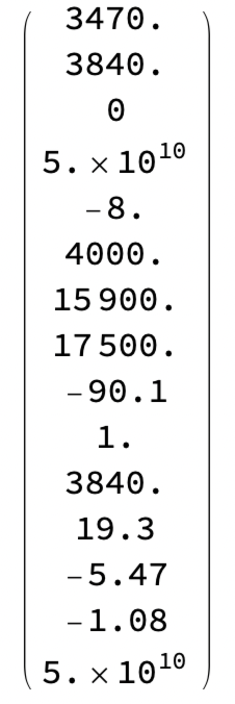
\includegraphics[width=0.2\textwidth]{SMProduct.pdf}
    \caption{Product of the Matrix A by the Unitary Vector}
    \label{fig:sparsematrixproductz}
\end{figure}

Comparing this result with the one obtained by numpy dot function, it is clear that the function is working properly. 